\chapter{Histograma de orientação de gradientes para poses de mão em um ambiente automotivo}

Esse capítulo tem como objetivo descrever as etapas da pesquisa prática. Conforme figura \ref{fig:research_steps} os principais passos do projeto são a construção da câmera infravermelha, a geração da base de dados, a seleção das imagens que servirão de treinamento para o classificador SVM e depois o cálculo do HOG em todas as imagens, variando os seus parâmetros e medindo o desempenho do algoritmo. Dessa forma é possível avaliar se a técnica proposta obteve uma boa resposta para as poses de mão e discutir quais as poses que melhor são representadas pela suas orientações do gradiente.

\begin{figure}[ht!]
	\centering
  	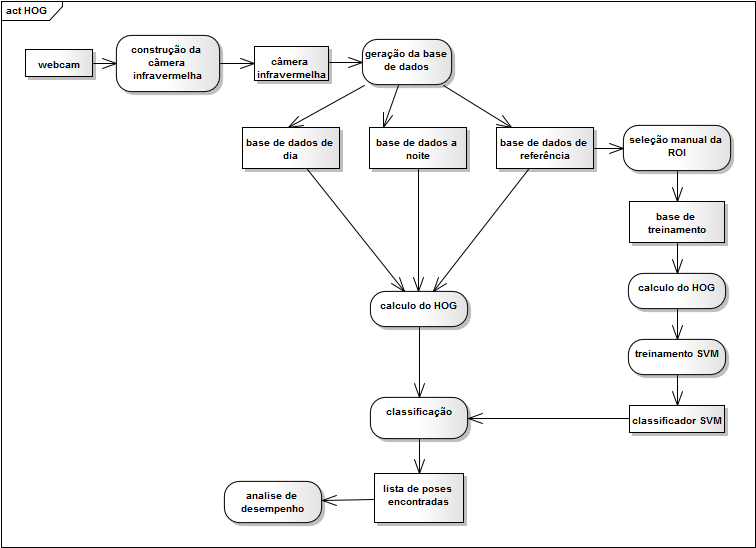
\includegraphics[scale=0.3]{image/HOG.png}
  	\caption{Fluxo de trabalho da pesquisa}
  	\label{fig:research_steps}
\end{figure}

\section{Construção da câmera infravermelha}

A câmera utilizada nessa aplicação tem que ser capaz de capturar imagens nas mais diversas condições de luminosidade. Temos o caso, por exemplo, de um dia de sol cuja intensidade de luz é bem alta. Até o ponto onde não há luz nenhuma.
Nesses casos é necessário uma iluminação própria, mas ao mesmo tempo, não pode atrapalhar o motorista. Por isso, a iluminação infra vermelha é muito utilizada. O custo é baixo e não interfere em nada no ambiente. O maior contratempo desse tipo de iluminação é que se perde toda a informação de cor.
Para gerar a base de dados para o nosso estudo, utilizamos uma câmera normal de mercado, modificada para receber a luz infra vermelha e colocamos LEDs de infra vermelho para fazer a iluminação.

\begin{figure}[ht!]
	\centering
	\setlength{\fboxsep}{1pt}
	\fbox{
  		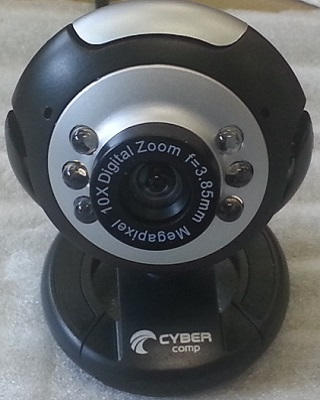
\includegraphics[scale=0.3]{image/webcam01.jpg}
 		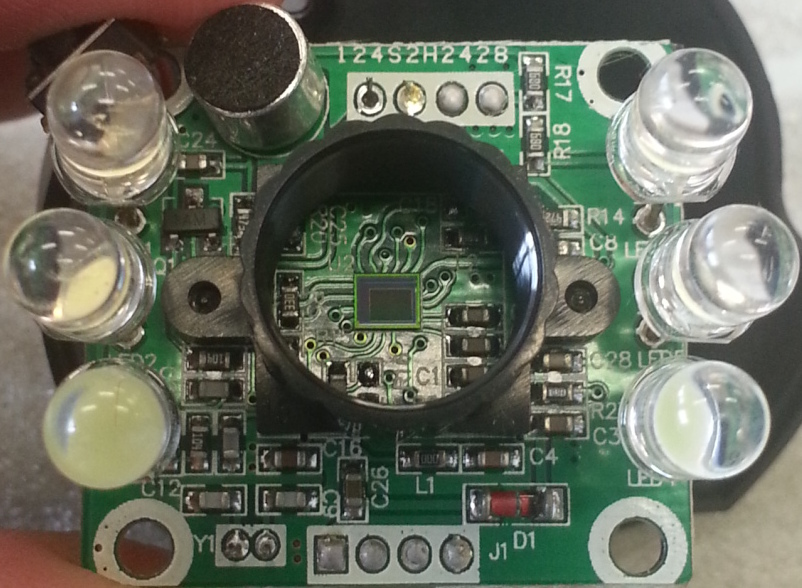
\includegraphics[scale=0.3]{image/webcam02.jpg}
 	}
  	\caption{Webcam utilizada na aquisição das imagens sem nenhuma modificação}
  	\label{fig:camera_01}
\end{figure}


Na figura \ref{fig:camera_01} temos a câmera utilizada para a aquisição das imagens. Nesse momento a câmera ainda não foi modificada. Essa câmera portanto ainda possui um filtro de luz infravermelha e os LEDs de iluminação são LEDs brancos.

A principal modificação a ser feita nesse tipo de câmera é retirar o filtro infravermelho. Esse filtro é uma placa de vidro localizada atrás da lente. Na figura \ref{fig:camera_02} temos uma foto das lentes ainda com o filtro e depois já com o filtro retirado. E preciso também substituir os LEDs atuais, que são LEDs brancos, para LEDs infra vermelho de 950nm.

\begin{figure}[ht!]
	\centering
	\setlength{\fboxsep}{1pt}
	\fbox{
		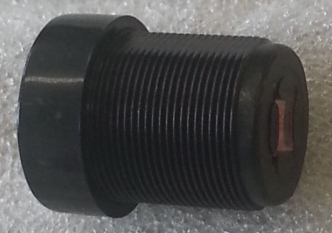
\includegraphics[width=0.3\textwidth]{image/webcam03.jpg}
  		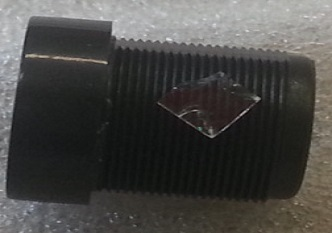
\includegraphics[width=0.3\textwidth]{image/webcam05.jpg}
  	}
  	\caption{Lentes com o filtro infra vermelho localizado na parte traseira}
  	\label{fig:camera_02}
\end{figure}

\section{Elaboração da base de dados}

As bases de dados que serão usadas no trabalho precisam refletir as condições que encontramos em um ambiente automotivo. Por isso elaboramos um conjunto de banco de imagens que variam o fundo, o usuário, a iluminação e a vestimenta. A resolução das imagens será 320x240 e a janela terá o tamanho de 120x110 pixeis.

O nosso fundo vai variar conforme o carro de onde as imagens foram coletadas. Como referência, temos também um conjunto de imagens com o fundo preto homogêneo.
O usuário será também modificado, variando sexo e cor de pele. A iluminação terá a captura diurna e noturna e a vestimenta varia por exemplo se o usuário esta usando blusa, relógio, etc.

Para o usuário temos a tabela \ref{table:usuarios} mostrando as suas principais características.

\begin{table}[h]
	\centering
	\begin{tabular}{|c|c|c|}
		\hline Usuário & Sexo & Cor de pele \\
		\hline 1 & Masculino & Branco \\
		\hline 2 & Masculino & Branco \\
		\hline 3 & Feminino & Branco \\
		\hline 4 & Masculino & Moreno \\
		\hline 5 & Feminino & Negra \\
		\hline
	\end{tabular}
	\caption{Lista de usuários}
	\label{table:usuarios}
\end{table}

A base de referência será um banco de imagens com o fundo preto homogêneo, o usuário 1 do sexo masculino sem nenhum tipo de vestimenta ou acessório e a iluminação apenas dos LEDs infravermelhos, ou seja, em um ambiente totalmente escuro. Na tabela \ref{table:data_base_1} temos um resumo da parametrização dessa base e alguns exemplos das imagens.

\newcommand{\adddb}[9]{
\begin{table}[H]
	\centering
	\begin{tabular}{c c}
	\begin{tabular}{|c|c|}
		\hline \textbf{Usuário} 	& #1	\\ 
		\hline \textbf{Fundo} 		& #2	\\ 
		\hline \textbf{Iluminação} 	& #3	\\
		\hline \textbf{Vestimenta} 	& #4	\\
		\hline 
	\end{tabular} 
	&
	\begin{tabular}{|c|c|c|}
		\hline 
			\multicolumn{3}{|c|}{Gestos} \\ 
		\hline
			\raisebox{-.5\height}{\includegraphics[scale=0.25]{#5}} & 
			\raisebox{-.5\height}{\includegraphics[scale=0.25]{#6}} & 
			\raisebox{-.5\height}{\includegraphics[scale=0.25]{#7}} \\ 
		\hline 
	\end{tabular}
	\\
	\end{tabular}

	\caption{#8}
	\label{#9}
\end{table}
}

\adddb{Usuário 1}{Preto homogêneo}{Infra vermelha}{Nenhuma}{image/ir_led_2/0_02.jpg}{image/ir_led_2/1_02.jpg}{image/ir_led_2/7_02.jpg}{Parametrização da base de referência (conjunto 1)}{table:data_base_1}

% ***********************************************

Na tabela \ref{table:data_base_2} tem-se um conjunto de imagens com o fundo do carro Ford Focus, iluminação com LEDs infravermelhos e usuário 1 com uma blusa preta.

\adddb{Usuário 1}{Ford Focus}{Infra vermelha}{Blusa preta}{image/night/focus/gustavo/blackshirt/0_02.jpg}{image/night/focus/gustavo/blackshirt/1_01.jpg}{image/night/focus/gustavo/blackshirt/7_01.jpg}{Parametrização do conjunto 2}{table:data_base_2}

% ***********************************************

Na tabela \ref{table:data_base_3} tem-se um conjunto de imagens com o fundo do carro Ford Focus, iluminação com LEDs infravermelhos e usuário 1 sem vestimentas.

\adddb{Usuário 1}{Ford Focus}{Infra vermelha}{Nenhuma}{image/night/focus/gustavo/shortshirt/0_02.jpg}{image/night/focus/gustavo/shortshirt/1_01.jpg}{image/night/focus/gustavo/shortshirt/7_01.jpg}{Parametrização do conjunto 3}{table:data_base_3}

% ***********************************************

Na tabela \ref{table:data_base_4} tem-se um conjunto de imagens com o fundo do carro Passat, iluminação com LEDs infravermelhos e usuário 2 usando uma blusa verde. O interessante desse conjunto é a existência de um LED no painel que pode atrapalhar a segmentação da imagem.

\adddb{Usuário 2}{Passat}{Infra vermelha}{Blusa verde}{image/night/passat/rogerio/blusaverde/0_02.jpg}{image/night/passat/rogerio/blusaverde/1_01.jpg}{image/night/passat/rogerio/blusaverde/7_01.jpg}{Parametrização do conjunto 4}{table:data_base_4}

\section{Treinamento}

Como visto anteriormente, na tabela \ref{table:dlal_hog}, o HOG é calculado usando células de 8x8 pixeis, agrupadas em blocos de 2x2 células. Portanto, se aplicado o HOG com os parâmetros originais em uma imagem de 320x240, tem-se 40x30 células. Cada célula contribui quatro vezes para a formação do vetor de características por conta na sobreposição que existe na normalização em blocos, com exceção das bordas, que contribuem apenas uma vez. Portanto, tem-se 40 + (40-2) x 30 + (30-2) células. Cada histograma tem 9 grupos de ângulos totalizando um vetor de 40.716 dimensões. Na figura \ref{fig:hog_example1} tem-se um exemplo visual do HOG. Cada histograma de cada célula é mostrado usando um diagrama de rosa. O tamanho de cada pétala do diagrama é ajustado para indicar a contribuição que aquela orientação representa no histograma da célula. 

\begin{figure}[H]
	\centering
	\begin{tabular}{p{0.5\textwidth} p{0.5\textwidth}}
		\vspace{1pt} 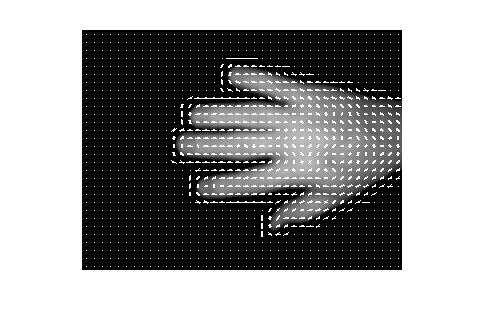
\includegraphics[width=0.6\textwidth]{image/hog/0_01.png} &
		\vspace{0pt} 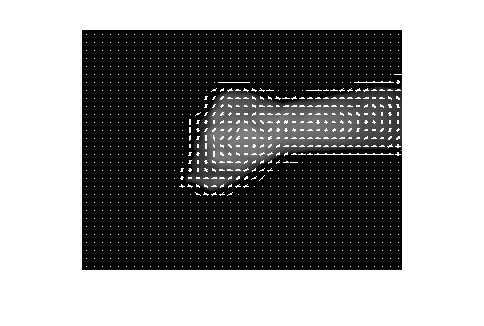
\includegraphics[width=0.6\textwidth]{image/hog/7_01.png}
	\end{tabular}	
  	\caption{Exemplos do cálculo do HOG com os parâmetros originais}
  	\label{fig:hog_example1}
\end{figure}

O banco de imagens possui exemplares de 12 poses diferentes. Cada imagem existente foi retirada manualmente de um vídeo, capturando diversos exemplares de cada pose de mão. Os arquivos criados seguiram uma metodologia de nomeação conforme o padrão \([pose]\_[número].jpg\). No qual \([pose]\) é o número da pose de mão conforme a tabela \ref{table:poses_mao} e \([número]\) é uma enumeração sequencial da pose para diferenciação das demais semelhantes.

\newcommand{\addpose}[2] {
	\arabic{table:counter_poses_mao} \stepcounter{table:counter_poses_mao} & 
	#1 & 
	\includegraphics[width=0.1\linewidth]{#2}
}

\begin{table}[H]
	\centering
	
	\begin{tabular}{|c|c|c|}
		\hline Número 	& Descrição 	& Imagem 	
		\newcounter{table:counter_poses_mao}						\\ 
		\hline \addpose{Mão aberta / 5 dedos}{image/hog/0_01.jpg}		\\
		\hline \addpose{1 dedo}{image/hog/1_01.jpg}		\\
		\hline \addpose{2 dedos}{image/hog/2_01.jpg}		\\
		\hline \addpose{3 dedos}{image/hog/3_01.jpg}		\\
		\hline \addpose{4 dedos}{image/hog/4_01.jpg}		\\
		\hline \addpose{Revólver}{image/hog/5_01.jpg}		\\
		\hline \addpose{Palma aberta}{image/hog/6_01.jpg}		\\
		\hline \addpose{Palma fechada}{image/hog/7_01.jpg}		\\
		\hline \addpose{OK}{image/hog/8_01.jpg}		\\
		\hline \addpose{Telefone}{image/hog/9_01.jpg}		\\
		\hline \addpose{Chifre}{image/hog/10_01.jpg}		\\
		\hline \addpose{Revólver com cano duplo}{image/hog/11_01.jpg}		\\
		\hline 
	\end{tabular} 
	
	\caption{Poses de mão utilizadas}
	\label{table:poses_mao}
\end{table}

Primeiramente, será criado um conjunto de classificadores SVM (Support Vector Machine) para cada pose de mão que a pesquisa abrange. Esse conjunto é formado por 3 classificadores com foco na variação da luminosidade. Um para as imagens feitas durante o dia, um outro para as imagens infra vermelhas feitas à noite e um terceiro que seria genérico tanto para dia quanto para noite. O intuito é testar se a performance de um classificador específico para a luminosidade é melhor do que um classificador que abrange os dois tipos.

As imagens de treinamento serão geradas manualmente extraindo uma janela (110x120) com a pose de mão correspondente da base de referência. 

Cada classificador será avaliado considerando imagens da pose versus imagens sem a pose e depois imagens da pose versus imagens de outras poses. Esse teste permite avaliar quais as poses são mais parecidas.

Considerando que temos 12 poses diferentes, teremos um total de 36 classificadores.
 
Depois um novo conjunto de classificadores será gerado (um para cada tipo de luminosidade) mas com treinamento de todas as poses com o objetivo de detectar mão independente da pose.

%O tempo de cálculo será medido para cada parâmetro avaliado, para %que depois se possa analisar o quão mais rápido o algoritmo se %torna conforme seu desempenho cai.

\section{Cálculo do HOG}

Para o cálculo do HOG será necessário a implementação do algoritmo como um todo. O MATLAB \cite{MATLAB:2013} possui uma implementação do mesmo mas com pouca liberdade para parametrização. Ele permite a mudança do tamanho da célula, o tamanho do bloco, a quantidade de sobreposição entre blocos, o número de grupos de ângulos no histograma e se o ângulo varia entre 0 á 180 ou 0 á 360. Mas não permite mudar a maneira com que os ângulos são classificados no histograma, o valor do gama, e nem o tipo de normalização. Portanto para se ter um controle melhor da variação dos parâmetros, a implementação é justificável

O cálculo será repetido variando os parâmetros conforme a tabela \ref{table:hog_var}.

\begin{table}[H]
	\centering
	\begin{tabular}{|c|c|}
	\hline
		Gama 					& 1, 1/2 				\\
	\hline  
		Número de células 		&  8x8 até 240x240 		\\ 
	\hline  
		Número de blocos  		&  2x2 e 1x1 			\\ 
	\hline 
		Tipo de normalização  	&  L2-norm, L2-Hys,  L1-norm , L1-sqrt 										\\ 
	\hline 
		Agrupamento dos ângulos	&  9 a 36				\\ 
	\hline
		Sinal dos ângulos		& 0-180 / 0-360			\\
	\hline		
	\end{tabular} 
	\caption{Resumo dos parâmetros que serão variados no cálculo do HOG}
	\label{table:hog_var}
\end{table}

\section{Análise dos resultados}

Para quantificar a performance dos classificadores que serão criados, optou-se pela geração de um gráfico do tipo DET (Detection Error Tradeoff). Esse tipo de gráfico é usado em classificações binárias medindo falso negativo vs. falso positivo em uma escala log-log. As curvas de gráficos do tipo DET tendem a ser mais lineares do que as curvas ROC (Receiver Operating Characteristics), facilitando a análise para pequenas variações. Os eixos serão: Taxa de Erro (\(FalsoNeg/VerdadeiroPos + FalsoNeg\)) versus Falso Positivo por Janela (FPPW do inglês False Positive per Window).

\chapter{Discussão}

O objetivo desse capítulo é discutir a relação entre a hipótese formulada no trabalho, a teoria existente sobre o assunto e a prática demonstrada no capítulo anterior, contribuindo com o estudo do \citeonline{dalal2006finding} parametrizando as poses de mão em um ambiente automotivo. A tabela \ref{table:key_hog} mostra a parametrização feita por \citeonline{dalal2006finding} para diversas classes de objetos.
Como as poses propostas por esse trabalho possuem formatos bastante distintos é possível que se chegue na conclusão que cada pose possua sua própria parametrização.

\begin{table}[H]
	\centering
	\begin{tabular}{|c|c|c|c|c|c|}
	\hline
		Classe & Tamanho da janela & Grupo de ângulos & Range & Gama & Normalização \\
	\hline  
		Pessoa & 64x128 & 9 & (0-180\degree) & \(\sqrt{RGB}\) & L2-Hys \\
	\hline  
		Carro & 104x56 & 18 & (0-360\degree) & \(\sqrt{RGB}\) & L1-Sqrt \\
	\hline  
		Moto & 120x80 & 18 & (0-360\degree) & \(\sqrt{RGB}\) & L1-Sqrt \\
	\hline  
		Ônibus & 120x80 & 18 & (0-360\degree) & \(\sqrt{RGB}\) & L1-Sqrt \\
	\hline  
		Bicicleta & 104x64 & 18 & (0-360\degree) & \(\sqrt{RGB}\) & L2-Hys \\
	\hline  
		Vaca & 128x80 & 18 & (0-360\degree) & \(\sqrt{RGB}\) & L2-Hys \\
	\hline  
		Ovelha & 104x60 & 18 & (0-360\degree) & \(\sqrt{RGB}\) & L2-Hys \\
	\hline  
		Cavalo & 128x80 & 9 & (0-180\degree) & \(RGB\) & L1-Sqrt \\
	\hline  
		Gato & 96x56 & 9 & (0-180\degree) & \(RGB\) & L1-Sqrt \\
	\hline  
		Cachorro & 96x56 & 9 & (0-180\degree) & \(RGB\) & L1-Sqrt \\
	\hline		
	\end{tabular} 
	\caption{Parametrização  para diferentes classes de objetos \cite{dalal2006finding}.}
	\label{table:key_hog}
\end{table}

\chapter{Conclusão}

A pesquisa mostra que a interação do homem com o seu veículo através de gestos é apenas uma questão de tempo e que existe uma gama gigantesca de técnicas e algoritmos que podem ser usados para o serviço. Um deles é o Histogram of Oriented Gradients (HOG), que tem mostrado uma grande robustez contra grandes variações de luminosidade e tem sido aplicado nas mais diferentes classes de objetos. Ele é recomendado para objetos cuja forma se mantem, mesmo em ângulos diferentes, que é o caso das poses de mão. Mesmo variando a pessoa ou a vestimenta, a forma de cada pose se mantem, diferentemente de um gato, por exemplo, que pode assumir diversas formas dependendo de como ele está posicionado. O gato pode estar dormindo todo esticado, ou todo enrolado dentro de uma caixa, pode estar andando ou de barriga para cima brincando. Essas grandes variações de formas para um mesmo tipo de objetivo não é o tipo recomendado para o uso do HOG.

É esperado que cada dedo da mão contribua de forma bastante significativa para o histograma de orientações com graus bastante uniformes, criando uma boa distinção em relação ao fundo do veículo.

A câmera infravermelha também tem mostrado uma solução eficaz de captura de imagens no escuro. Não é necessário uma grande quantidade de LEDs para poder fazer as aquisições da imagem e não se faz distinção para cor de peles diferentes ou caso se faça uso de luvas.

Por fim, o trabalho se encaminha para concluir um conjunto de parâmetros para melhor se calcular o HOG, criando assim, um descritor de poses de mão para aplicações automotivas. E também, determinar as melhores poses de mão para a aplicação proposta.

\chapter{Cronograma}

Esse capítulo apresenta o cronograma do trabalho, descrevendo as etapas do projeto e seus progressos.

Como tarefas em andamento ou planejadas para execução temos: Referência bibliográfica, que visa o acompanhamento das publicações mais atuais do tema e apoio para teorização da parte prática que será desenvolvida. Elaboração da base de dados dia, que visa a construção de uma banco de imagens que contemple as poses discutidas no trabalho no interior do veículo durante o dia, ou seja, com iluminação natural. Preparação das imagens de treinamento, que visa o trabalho manual de classificar, recortar e centralizar as poses de mão dentro da imagem original. Implementação do algoritmo, que visa desenvolver de forma parametrizável cada etapa do HOG. Aplicação do algoritmo, que visa exercitar a implementação para o banco de imagens criado. E por fim, análise dos resultados, que visa analisar e concluir os resultados dos experimentos. 

\noindent\resizebox{\textwidth} {!} {
\begin{ganttchart}[
				       vgrid,								% Add vertical lines in the bar canvas
				       bar/.append style={fill=blue!50},	% By default, fill bars with blue color
				       progress=today,						% Add progress information
				       today=3,								% Today configuration (month # * 2)
				  ] {1}{14}
\gantttitle{2014}{10} 						
\gantttitle{2015}{4} 						\\
\gantttitlelist{8,9,10,11,12,1,2}{2} 		\\

% Tasks
\ganttbar{Referência bibliográfica}{1}{12} 					\\
\ganttbar{Preparação para qualificação}{2}{3} 				\\
\ganttmilestone[progress=none]{Qualificação}{3} 			\ganttnewline
\ganttbar{Elaboração da base de dados dia}{4}{6} 			\\
\ganttbar{Preparação das imagens de treinamento}{5}{6}		\\
\ganttbar{Implementação do algoritmo}{7}{8}					\ganttnewline
\ganttbar{Aplicação do algoritmo}{9}{10} 					\\
\ganttbar{Análise dos resultados}{11}{12} 					\\
\ganttmilestone[progress=none]{Banca final}{13}				
\end{ganttchart}
}